% =============================================================================
%  lec03.tex —— 第 3 讲 单纯集（底本 PDF 第 16–27 页）
% =============================================================================
\lecture{3}{单纯集}
\begin{center}\small\color{black!55}（底本 PDF 第 16–27 页）\end{center}

本讲的目标是介绍拓扑空间同伦论的一种组合进路，即\textbf{单纯集的 Kan--Quillen 模型范畴}。

\section{单纯集}

\begin{definition}\label{L3-1.1}
对 $n\in\Z_{\ge 0}$，令
\[
[n]\defeq\{0<1<\cdots<n\}
\]
为具有 $(n+1)$ 个对象的全序集。按通常方式把它视为范畴。
\end{definition}

\begin{definition}\label{L3-1.2}
\textbf{单纯范畴} $\Delta$ 是 $\Cat$ 的由 $[n]\in\Cat$（$n\in\Z_{\ge 0}$）构成的全子范畴；换言之，$\Hom_{\Delta}([m],[n])$ 是全体非减函数 $[m]\to[n]$ 构成的集合。

令 $\Delta_{\mathrm{inj}}$ 与 $\Delta_{\mathrm{surj}}$ 分别为 $\Delta$ 的由单射态射与满射态射构成的子范畴。
\end{definition}

\nitem\label{L3-1.3}
设 $\cC$ 是范畴。则 $\Hom_{\Cat}([n],\cC)$ 与 $\cC$ 中长度为 $n$ 的链构成的集合等价。

单纯范畴 $\Delta$ 在范畴论中无处不在，这一点可由下述结果解释。

\begin{proposition}\label{L3-1.4}
函子
\begin{equation}\label{L3-eq1.1}
\Cat\to\Fun(\Delta^{\op},\Set),\qquad \cC\mapsto\Hom_{\Cat}(-,\cC)
\end{equation}
是全忠实的。
\end{proposition}

\begin{definition}\label{L3-1.5}
设 $\cD$ 是范畴。
\begin{itemize}[leftmargin=2.2em,itemsep=0.1em]
\item $\cD$ 的一个\textbf{单纯对象}是函子 $\Delta^{\op}\to\cD$。
\item $\cD$ 的一个\textbf{余单纯对象}是函子 $\Delta\to\cD$。
\end{itemize}
\end{definition}

\nitem\label{L3-1.6}
设 $X$ 是单纯对象，我们常写 $X_{n}\defeq X([n])$，从而也把这个单纯对象记作 $X_{\bullet}$。类似地，余单纯对象常记作 $Y^{\bullet}$。

\begin{definition}\label{L3-1.7}
记
\[
\Set_{\Delta}\defeq\Fun(\Delta^{\op},\Set)
\]
为单纯集范畴。
\end{definition}

\begin{example}\label{L3-1.8}
可表函子
\[
\Hom_{\Delta}(-,[n])\colon\Delta^{\op}\to\Set
\]
定义了一个单纯集 $\Delta^{n}$，称为 $n$-\textbf{单形}。
\end{example}

\nitem\label{L3-1.9}
设 $X$ 是单纯集。由 Yoneda 引理，有
\[
\Hom_{\Set_{\Delta}}(\Delta^{n},X)\simeq X_{n}.
\]
这促成了下述定义：

\begin{definition}\label{L3-1.10}
设 $X_{\bullet}$ 是单纯集。元素 $x\in X_{n}$ 称为 $X$ 的一个 $n$-\textbf{单形}。
\end{definition}

\begin{definition}\label{L3-1.11}
设
\[
\mathbf{N}_{\bullet}\colon\Cat\to\Set_{\Delta}
\]
为函子~\eqref{L3-eq1.1}。对范畴 $\cC$，单纯集 $\mathbf{N}_{\bullet}(\cC)$ 称为 $\cC$ 的\textbf{脉}。
\end{definition}

\yizhu{nerve 字面意为“神经”，中译数学文献通行作“脉”，故 nerve functor 译“脉函子”、simplicial nerve 译“单纯脉”，此处从 glossary 统一。\textbf{[来源：B]}}

\nitem\label{L3-1.12}
命题~\ref{L3-1.4} 说，范畴的理论可以通过构造 $\cC\mapsto\mathbf{N}_{\bullet}(\cC)$ 嵌入单纯集的理论。因此，

\begin{slogan}\label{L3-1.13}\centering\par
单纯集推广了范畴。
\end{slogan}

\begin{construction}\label{L3-1.14}
对合 $(-)^{\op}\colon\Cat\to\Cat$ 限制为对合 $(-)^{\op}\colon\Delta\to\Delta$，后者诱导对合
\[
(-)^{\op}\colon\Set_{\Delta}\to\Set_{\Delta}.
\]
\end{construction}

\begin{exercise}\label{L3-1.15}
脉函子 $\mathbf{N}_{\bullet}\colon\Cat\to\Set_{\Delta}$ 与取反范畴/反单纯集相容。
\end{exercise}

\section{面与退化}

\begin{definition}\label{L3-2.1}
对 $n>0$，令
\[
\delta^{i}_{n}\colon[n-1]\to[n]
\]
为唯一的使 $i\in[n]$ 不在像中的函子。

设 $X$ 是范畴 $\cD$ 中的单纯对象。$X_{n}$ 上的第 $i$ 个\textbf{面算子}是态射
\[
d^{n}_{i}\defeq X(\delta^{i}_{n})\colon X_{n}\to X_{n-1}.
\]
\end{definition}

\begin{definition}\label{L3-2.2}
设 $X$ 是单纯集，$x\in X_{n}$ 是 $n$-单形。$(n-1)$-单形 $d^{n}_{i}(x)$ 称为 $x$ 的第 $i$ 个\textbf{面}。

更一般地，对任意单射函子 $\iota\colon[m]\to[n]$，$m$-单形 $X(\iota)(x)$ 称为 $x$ 的 $\iota$-\textbf{面}。
\end{definition}

\begin{definition}\label{L3-2.3}
对 $n\ge 0$，令
\[
\sigma^{i}_{n}\colon[n+1]\to[n]
\]
为唯一的在 $\{i,i+1\}$ 上取常值的满射函子。

设 $X$ 是范畴 $\cD$ 中的单纯对象。$X_{n}$ 上的第 $i$ 个\textbf{退化算子}是态射
\[
s^{n}_{i}\defeq X(\sigma^{i}_{n})\colon X_{n}\to X_{n+1}.
\]
\end{definition}

\begin{definition}\label{L3-2.4}
设 $X$ 是单纯集，$x\in X_{n}$ 是 $n$-单形。$(n+1)$-单形 $s^{n}_{i}(x)$ 称为 $x$ 的第 $i$ 个\textbf{退化}。

更一般地，对任意满射函子 $\pi\colon[m]\to[n]$，$m$-单形 $X(\pi)(x)$ 称为 $x$ 的 $\pi$-\textbf{退化}。
\end{definition}

\begin{definition}\label{L3-2.5}
设 $X$ 是单纯集，$x\in X_{n}$ 是 $n$-单形。若 $x$ 不是任何 $m<n$ 的 $m$-单形的退化，则称 $x$ 是\textbf{非退化的}。
\end{definition}

\begin{lemma}\label{L3-2.6}
任一退化单形都是某个非退化单形 $x$ 的 $\pi$-退化，且对 $(\pi,x)$ 唯一。
\end{lemma}

\begin{exercise}\label{L3-2.7}
$\Delta$ 中任一态射都等于若干 $\delta$ 与 $\sigma$ 的复合。
\end{exercise}

\begin{remark}\label{L3-2.8}
由此，知道单纯对象 $X_{\bullet}$ 等价于知道对象 $X_{n}$ 与满足某些关系的态射 $d^{n}_{i}$、$s^{n}_{i}$。这些关系称为\textbf{单纯恒等式}，可以显式写出：
\[
\begin{aligned}
d_{i}\circ d_{j}&=d_{j-1}\circ d_{i}, && i<j;\\
s_{i}\circ s_{j}&=s_{j}\circ s_{i-1}, && i>j;\\
d_{i}\circ s_{j}&=
\begin{cases}
s_{j-1}\circ d_{i}, & i<j,\\
\id, & i=j,\,j+1,\\
s_{j}\circ d_{i-1}, & i>j+1.
\end{cases}
\end{aligned}
\]
这里我们在记号中省略了上标。
\end{remark}

\nitem\label{L3-2.9}
我们可以把面态射与退化态射描成一个图
\begin{center}
\begin{tikzcd}[column sep=3.4em,row sep=1.1em]
X_{0}\arrow[r,shift left=0.45ex]\arrow[r,shift right=0.45ex] & X_{1}
\arrow[r,shift left=1.35ex]\arrow[r,shift left=0.45ex]\arrow[r,shift right=0.45ex]\arrow[r,shift right=1.35ex]
& X_{2}\arrow[r] & \cdots
\end{tikzcd}
\end{center}
有时人们省略退化态射，而用
\begin{center}
\begin{tikzcd}[column sep=3.4em,row sep=1.1em]
X_{0}\arrow[r,shift left=0.45ex]\arrow[r,shift right=0.45ex] & X_{1}
\arrow[r,shift left=0.45ex]\arrow[r,shift right=0.45ex] & X_{2}\arrow[r] & \cdots
\end{tikzcd}
\end{center}
来表示一个单纯对象，特别是在研究该图的\emph{余极限}时\footnote{在后续几讲中，我们将证明退化态射不影响单纯对象的 $\infty$-余极限/同伦余极限。}。

\begin{exercise}\label{L3-2.10}
设 $X$ 是单纯集。描述反单纯集 $X^{\op}$ 的面算子与退化算子。
\end{exercise}

\section{维数与骨架}

\begin{definition}\label{L3-3.1}
设 $X$ 是单纯集，$k\in\Z$。若对 $n>k$，$X$ 的每个 $n$-单形都是退化的，则称 $X$ 的\textbf{维数} $\le k$，记作 $\dim(X)\le k$。
\end{definition}

\begin{example}\label{L3-3.2}
$\dim(\Delta^{n})=n$。
\end{example}

\begin{definition}\label{L3-3.3}
设 $X$ 是单纯集，$k\in\Z$。$X$ 的 $k$-\textbf{骨架} $\mathrm{sk}_{k}(X)$ 是 $X$ 的维数 $\le k$ 的最大单纯子集。
\end{definition}

\section{例子}

\nitem\label{L3-4.1}
我们首先介绍画单纯集 $X_{\bullet}$ 的标准方式，这也是人们实际思考它们的方式。
\begin{itemize}[leftmargin=2.2em,itemsep=0.1em]
\item 只画非退化单形。退化单形按引理~\ref{L3-2.6} 的意义“塌缩”到与之对应的非退化单形上。
\item[]\hspace*{0.8em}(0) 对每个 $v\in X_{0}$，画一个标有 $v$ 的顶点。
\item[]\hspace*{0.8em}(1) 对每个非退化 $e\in X_{1}$，画一个标有 $e$ 的箭头，从 $d^{1}_{0}(e)$ 指向 $d^{1}_{1}(e)$。
\item[]\hspace*{0.8em}($n$) 对每个非退化 $\sigma\in X_{n}$，画一个标有 $\sigma$ 的实心 $n$-单形，其边界由 $d^{n}_{0}(\sigma),d^{n}_{1}(\sigma),\dots,d^{n}_{n}(\sigma)$ 给出\footnote{注意这些面可以是退化的。}。
\item 必要时，在单形内部写下符号以指示其顶点的次序。
\end{itemize}

\begin{exercise}\label{L3-4.2}
找出 $\Delta^{n}$ 中所有非退化单形。
\end{exercise}

\begin{center}
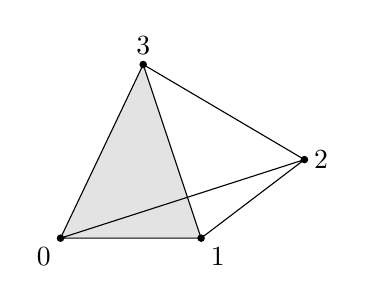
\begin{tikzpicture}[scale=1.05]
\coordinate (A) at (0,0); \coordinate (B) at (1.7,0); \coordinate (C) at (2.95,0.95); \coordinate (D) at (1.0,2.1);
\fill[gray!22] (A)--(B)--(D)--cycle;
\draw (A)--(B)--(C)--cycle;
\draw (A)--(D); \draw (B)--(D); \draw (C)--(D);
\foreach \P in {A,B,C,D} {\fill (\P) circle (1.3pt);}
\node[below left] at (A) {0}; \node[below right] at (B) {1};
\node[right] at (C) {2}; \node[above] at (D) {3};
\end{tikzpicture}
\par\smallskip{\small 图 1\quad 3-单形 $\Delta^{3}$}
\end{center}

\begin{exercise}\label{L3-4.3}
设 $\Delta^{1}\times\Delta^{1}$ 是 $\Set_{\Delta}$ 中的乘积。找出 $\Delta^{1}\times\Delta^{1}$ 中所有非退化单形。
\end{exercise}

\begin{center}
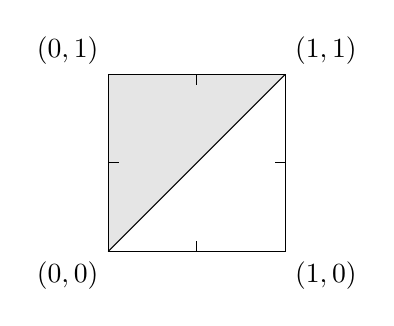
\begin{tikzpicture}[scale=1.5]
\fill[gray!20] (0,0)--(1.5,1.5)--(0,1.5)--cycle;
\draw (0,0) rectangle (1.5,1.5);
\draw (0,0)--(1.5,1.5);
\draw (0.75,0)--(0.75,0.09); \draw (0.75,1.5)--(0.75,1.41);
\draw (0,0.75)--(0.09,0.75); \draw (1.5,0.75)--(1.41,0.75);
\node[below left] at (0,0) {$(0,0)$};
\node[below right] at (1.5,0) {$(1,0)$};
\node[above right] at (1.5,1.5) {$(1,1)$};
\node[above left] at (0,1.5) {$(0,1)$};
\end{tikzpicture}
\par\smallskip{\small 图 2\quad 乘积 $\Delta^{1}\times\Delta^{1}$}
\end{center}

\begin{exercise}\label{L3-4.4}
在上例中，若在单纯集的定义中不允许退化，即把 $\Delta$ 换成 $\Delta_{\mathrm{inj}}$，会发生什么？
\end{exercise}

\begin{example}\label{L3-4.5}
令
\[
\partial\Delta^{n}\defeq\mathrm{sk}_{n-1}(\Delta^{n})
\]
为 $\Delta^{n}$ 的 $(n-1)$-骨架。我们称它为 $\Delta^{n}$ 的\textbf{边界}。
\end{example}

\begin{center}
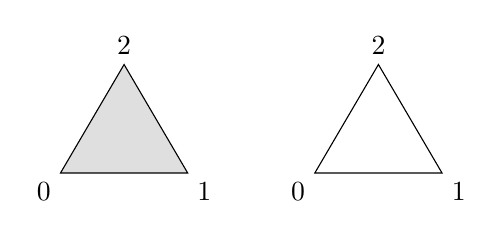
\begin{tikzpicture}[scale=0.95]
\fill[gray!25] (0,0)--(1.7,0)--(0.85,1.45)--cycle;
\draw (0,0)--(1.7,0)--(0.85,1.45)--cycle;
\node[below left] at (0,0) {0}; \node[below right] at (1.7,0) {1}; \node[above] at (0.85,1.45) {2};
\begin{scope}[xshift=3.4cm]
\draw (0,0)--(1.7,0)--(0.85,1.45)--cycle;
\node[below left] at (0,0) {0}; \node[below right] at (1.7,0) {1}; \node[above] at (0.85,1.45) {2};
\end{scope}
\end{tikzpicture}
\par\smallskip{\small 图 3\quad 2-单形 $\Delta^{2}$ 及其边界 $\partial\Delta^{2}$}
\end{center}

\begin{example}\label{L3-4.6}
令 $\Lambda^{n}_{i}$ 为 $\Delta^{n}$ 的不包含唯一非退化 $n$-单形的第 $i$ 个面的最大单纯子集。我们称它为 $\Delta^{n}$ 的第 $i$ 个\textbf{角}。
\end{example}

\begin{center}
\begin{tikzpicture}[scale=0.85]
\begin{scope}
\draw (0,0)--(1.5,0); \draw (0,0)--(0.75,1.25);
\node[below left] at (0,0) {0}; \node[below right] at (1.5,0) {1}; \node[above] at (0.75,1.25) {2};
\node[below] at (0.75,-0.75) {$\Lambda^{2}_{0}$};
\end{scope}
\begin{scope}[xshift=2.6cm]
\draw (0,0)--(1.5,0); \draw (1.5,0)--(0.75,1.25);
\node[below left] at (0,0) {0}; \node[below right] at (1.5,0) {1}; \node[above] at (0.75,1.25) {2};
\node[below] at (0.75,-0.75) {$\Lambda^{2}_{1}$};
\end{scope}
\begin{scope}[xshift=5.2cm]
\draw (0,0)--(0.75,1.25); \draw (1.5,0)--(0.75,1.25);
\node[below left] at (0,0) {0}; \node[below right] at (1.5,0) {1}; \node[above] at (0.75,1.25) {2};
\node[below] at (0.75,-0.75) {$\Lambda^{2}_{2}$};
\end{scope}
\end{tikzpicture}
\par\smallskip{\small 图 4\quad 角 $\Lambda^{2}_{0},\Lambda^{2}_{1},\Lambda^{2}_{2}$}
\end{center}

\nitem\label{L3-4.7}
读者可以用下述练习自娱，以检验对定义的理解。

\begin{exercise}\label{L3-4.8}
分类 $\Delta^{2}$ 的所有单纯商集，即在 $\Set_{\Delta}$ 中配有满射 $\Delta^{2}\to X$ 的单纯集 $X$。提示：共有 31 个。
\end{exercise}

\begin{center}
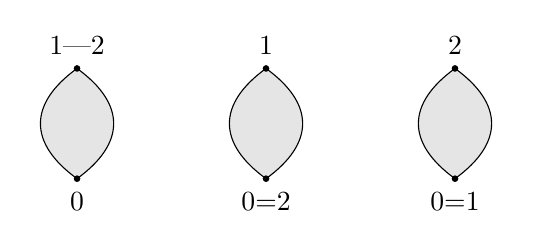
\begin{tikzpicture}[scale=1.0]
\begin{scope}
\fill[gray!20] (0,0) .. controls (-0.62,0.45) and (-0.62,0.95) .. (0,1.4) .. controls (0.62,0.95) and (0.62,0.45) .. (0,0);
\draw (0,0) .. controls (-0.62,0.45) and (-0.62,0.95) .. (0,1.4) .. controls (0.62,0.95) and (0.62,0.45) .. (0,0);
\fill (0,0) circle (1.2pt); \fill (0,1.4) circle (1.2pt);
\node[below] at (0,-0.05) {0}; \node[above] at (0,1.45) {1\text{—}2};
\end{scope}
\begin{scope}[xshift=2.4cm]
\fill[gray!20] (0,0) .. controls (-0.62,0.45) and (-0.62,0.95) .. (0,1.4) .. controls (0.62,0.95) and (0.62,0.45) .. (0,0);
\draw (0,0) .. controls (-0.62,0.45) and (-0.62,0.95) .. (0,1.4) .. controls (0.62,0.95) and (0.62,0.45) .. (0,0);
\fill (0,0) circle (1.2pt); \fill (0,1.4) circle (1.2pt);
\node[below] at (0,-0.05) {0=2}; \node[above] at (0,1.45) {1};
\end{scope}
\begin{scope}[xshift=4.8cm]
\fill[gray!20] (0,0) .. controls (-0.62,0.45) and (-0.62,0.95) .. (0,1.4) .. controls (0.62,0.95) and (0.62,0.45) .. (0,0);
\draw (0,0) .. controls (-0.62,0.45) and (-0.62,0.95) .. (0,1.4) .. controls (0.62,0.95) and (0.62,0.45) .. (0,0);
\fill (0,0) circle (1.2pt); \fill (0,1.4) circle (1.2pt);
\node[below] at (0,-0.05) {0=1}; \node[above] at (0,1.45) {2};
\end{scope}
\end{tikzpicture}
\par\smallskip{\small 图 5\quad $\Delta^{2}$ 的某些商}
\end{center}

\section{单纯集与拓扑空间}

\nitem\label{L3-5.1}
单纯范畴 $\Delta$ 可以如下实现为 $\Top$ 的子范畴。

\begin{construction}\label{L3-5.2}
令
\[
|\Delta^{n}|\defeq\{(x_{0},\dots,x_{n})\in\R^{n+1}_{\ge 0}\mid x_{0}+\cdots+x_{n}=1\}
\]
为标准（拓扑）$n$-单形。我们有函子
\begin{equation}\label{L3-eq5.1}
\Delta\to\Top,\qquad [n]\mapsto|\Delta^{n}|
\end{equation}
它把函子 $f\colon[m]\to[n]$ 送到连续映射
\[
|\Delta^{m}|\to|\Delta^{n}|,\qquad
(y_{0},\dots,y_{m})\mapsto\Bigl(\sum_{j\in f^{-1}(0)}y_{j},\dots,\sum_{j\in f^{-1}(n)}y_{j}\Bigr).
\]
\end{construction}

\begin{proposition}\label{L3-5.3}
我们通过 Yoneda 嵌入把 $\Delta$ 视为 $\Set_{\Delta}$ 的全子范畴。则函子~\eqref{L3-eq5.1} 可以延拓为保余极限的函子
\[
|-|\colon\Set_{\Delta}\to\Top,
\]
它在唯一等价的意义下唯一。我们称它为\textbf{几何实现}函子。

该函子有右伴随，由
\[
\Sing\colon\Top\to\Set_{\Delta},\qquad X\mapsto\Hom_{\Top}(|\Delta^{\bullet}|,X)
\]
给出。我们称它为\textbf{奇异单纯复形}函子\footnote{更好的名字是奇异单纯集函子，因为我们允许退化。}。
\end{proposition}

\nitem\label{L3-5.4}
伴随对
\[
|-|\colon\Set_{\Delta}\rightleftarrows\Top:\Sing
\]
属于范畴论中的下述范式。

\begin{exercise}\label{L3-5.5}
设 $\cC_{0}$ 是小范畴。定义 $\cC_{0}$ 上的\textbf{预层范畴}为
\[
\mathrm{PShv}(\cC_{0})\defeq\Fun(\cC_{0}^{\op},\Set).
\]
\begin{enumerate}[label=(\arabic*),leftmargin=2.4em,itemsep=0.1em]
\item 证明 $\mathrm{PShv}(\cC_{0})$ 是由 $\cC_{0}$ 在小余极限下自由生成的范畴。换言之，对任意含全体小余极限的范畴 $\cD$，Yoneda 嵌入 $\cC_{0}\to\mathrm{PShv}(\cC_{0})$ 诱导等价
\[
\mathrm{LFun}(\mathrm{PShv}(\cC_{0}),\cD)\simeq\Fun(\cC_{0},\cD),
\]
其中 $\mathrm{LFun}(-,-)\subset\Fun(-,-)$ 由保余极限的函子组成。
\item 设 $F\colon\mathrm{PShv}(\cC_{0})\to\cD$ 是延拓 $F_{0}\colon\cC_{0}\to\cD$ 的保余极限函子。证明 $F$ 有右伴随，由
\[
G\colon\cD\to\mathrm{PShv}(\cC_{0}),\qquad d\mapsto\Hom_{\cD}(F_{0}(-),d)
\]
给出。
\end{enumerate}
\end{exercise}

\begin{exercise}\label{L3-5.6}
挑战：对函子 $\Delta\to\Cat$ 应用上述范式，构造伴随对 $L\colon\Set_{\Delta}\rightleftarrows\Cat:R$。描述 §4 中的单纯集在该函子下的像。
\end{exercise}

\nitem\label{L3-5.7}
与脉函子 $\mathbf{N}_{\bullet}\colon\Cat\to\Set_{\Delta}$ 不同，函子 $\Sing\colon\Top\to\Set_{\Delta}$ 不是全忠实的。因此我们无法把拓扑空间的理论嵌入单纯集的理论。尽管如此，下述由 Quillen 在 1960 年代建立的结果（见 [Qui67]）说，二者的同伦论是相同的。

\begin{theorem}[Quillen]\label{L3-5.8}
伴随对
\[
|-|\colon\Set_{\Delta}\rightleftarrows\Top:\Sing
\]
诱导拓扑空间与单纯集的同伦论之间的等价。
\end{theorem}

\section{$\Set_{\Delta}$ 上的经典模型结构}

\nitem\label{L3-6.1}
为解释 Quillen 的结果，我们需要先定义 $\Set_{\Delta}$ 上的模型结构。

\begin{theoremdef}\label{L3-6.2}
$\Set_{\Delta}$ 上存在一个模型结构，由以下给出：
\begin{itemize}[leftmargin=3.4em,itemsep=0.15em]
\item [(W)] \textbf{弱同伦等价}是态射 $f\colon X\to Y$，使得
$|f|\colon|X_{\bullet}|\to|Y_{\bullet}|$ 是弱同伦等价。
\item [(C)] \textbf{上纤维化}是单态射。
\item [(F)] \textbf{Kan 纤维化}是态射 $f\colon X\to Y$，它对所有角包含 $\Lambda^{n}_{i}\to\Delta^{n}$（$0\le i\le n$、$n\ge 2$）具有右提升性质：
\begin{center}
\begin{tikzcd}[column sep=3.4em,row sep=2.6em]
\Lambda^{n}_{i}\arrow[r]\arrow[d,hook]\arrow[dr,dashed] & X\arrow[d,"f"]\\
\Delta^{n}\arrow[r] & Y.
\end{tikzcd}
\end{center}
\end{itemize}
我们称它为 $\Set_{\Delta}$ 上的\textbf{经典}模型结构，或 \textbf{Kan--Quillen 模型结构}。

该模型范畴中的纤维对象称为 \textbf{Kan 复形}。令 $\Kan\subset\Set_{\Delta}$ 为由 Kan 复形构成的全子范畴。
\end{theoremdef}

\begin{exercise}\label{L3-6.3}
找出 $\Delta^{1}$ 的一个纤维替换，即一个弱同伦等价 $\Delta^{1}\to X$，其中 $X$ 是 Kan 复形。
\end{exercise}

\begin{exercise}\label{L3-6.4}
找出 $\partial\Delta^{2}$ 的一个纤维替换。
\end{exercise}

\begin{exercise}\label{L3-6.5}
挑战：对 Kan 复形 $X$，在 $\Set_{\Delta}[W^{-1}]$ 中构造 $X$ 与 $X^{\op}$ 之间的典范同构。提示：扭曲箭头。
\end{exercise}

\begin{remark}\label{L3-6.6}
可以不用几何实现函子来定义单纯集之间的弱同伦等价。我们这样定义：
\begin{itemize}[leftmargin=3.4em,itemsep=0.15em]
\item [(W)] \textbf{弱同伦等价}是态射 $f\colon X\to Y$，使得对任意 Kan 复形 $Z$，映射
\[
[Y,Z]\to[X,Z]
\]
是双射，其中集合 $[X,Z]$ 是
\[
\Hom_{\Set_{\Delta}}(X\times\Delta^{1},Z)\rightrightarrows\Hom_{\Set_{\Delta}}(X,Z)
\]
的余等化子。
\end{itemize}
由 Quillen 定理~\ref{L3-5.8}（其精确形式见定理~\ref{L3-8.1}）与 Yoneda 引理，这两个定义事后是等价的。然而，选这一个定义还是那一个，会显著影响检验模型范畴公理与证明 Quillen 定理的方式。对本课程而言，这些证明被当作黑箱，读者不妨把两种陈述都当作定义。
\end{remark}

\section{同伦论之间的等价}

\nitem\label{L3-7.1}
本节解释两个同伦论之间等价的意义。设 $F\colon\cC\rightleftarrows\cD:G$ 是模型范畴之间的伴随对\footnote{我们不要求 $F$ 或 $G$ 保持 (W) 或 (C) 或 (F)。}。我们需要回答下述问题：
\begin{center}
\emph{这个伴随对何时诱导 $\cC$ 与 $\cD$ 底层的同伦论之间的等价？}
\end{center}
答案将是
\begin{itemize}[leftmargin=2.2em,itemsep=0.1em]
\item 伴随对 $F\colon\cC\rightleftarrows\cD:G$ 应诱导伴随对
\[
F^{\prime}\colon\cC[W^{-1}]\rightleftarrows\cD[W^{-1}]:G^{\prime},
\]
使得 $F^{\prime}$ 与 $G^{\prime}$ 互为逆\footnote{经典术语是拟逆（quasi-inverse），即要求 $\id\to G^{\prime}\circ F^{\prime}$ 与 $F^{\prime}\circ G^{\prime}\to\id$ 是等价而非相等。后一要求违背等价原则，因而在高阶范畴论中没有意义。因此我们省去前缀“拟”。}。
\end{itemize}
然而，要让它有意义，我们需要说清函子 $F^{\prime}$ 与 $G^{\prime}$ 的定义。这样一个定义的试金石是下述来自同调代数的例子。

\begin{example}\label{L3-7.2}
设 $A_{i}$ 是 Abel 范畴，使得 $\Ch^{\le 0}(A_{i})$ 上的投射模型结构有良好定义（见第 2 讲例 2.7）。我们有
\[
\Ch^{\le 0}(A_{i})[W^{-1}]\simeq\mathrm{D}^{\le 0}(A_{i}),
\]
其中 $\mathrm{D}^{\le 0}(A_{i})$ 是 $A_{i}$ 的导出范畴的连通（＝非正）部分。设 $F_{0}\colon A_{1}\to A_{2}$ 是加性函子，并考虑由 $F_{0}$ 诱导的函子
\[
F\colon\Ch^{\le 0}(A_{1})\to\Ch^{\le 0}(A_{2}).
\]
则我们希望 $F^{\prime}$ 是\textbf{左导出函子} $\mathbb{L}F$，它可由
\[
\mathbb{L}F(M^{\bullet})\simeq F(P^{\bullet})
\]
计算，其中 $P^{\bullet}\to M^{\bullet}$ 是 $M^{\bullet}$ 的上纤维替换，亦即投射消解。

需要对函子 $F_{0}$ 作额外假设，才能保证 $F(P^{\bullet})\in\mathrm{D}^{\le 0}(A_{2})$ 不依赖 $P^{\bullet}$ 的选取。
\end{example}

\begin{example}\label{L3-7.3}
对偶地，对单射模型范畴 $\Ch^{\ge 0}(A_{i})$，我们希望恢复\textbf{右导出函子}的定义。
\end{example}

\nitem\label{L3-7.4}
注意在上例中，函子 $F$ 不保持拟同构（因为 $F_{0}$ 不正合）。因此在 §7.1 的一般框架下，我们不应当要求 $F$ 或 $G$ 保持\emph{所有}对象之间的弱等价。特别地，我们不能指望下述图交换：
\begin{center}
\begin{tikzcd}[column sep=4.6em,row sep=2.4em]
\cC\arrow[r]\arrow[d,"F"'] & \cC[W^{-1}]\arrow[d,"F^{\prime}"]\\
\cD\arrow[r] & \cD[W^{-1}]
\end{tikzcd}
\end{center}
不过，在同调代数中，导出函子给出了这种交换方形的最佳逼近。为解释其含义，我们需要一些定义。

\begin{definition}\label{L3-7.5}
设 $\pi\colon\cC\to\cC^{\prime}$ 是范畴之间的函子。对任意范畴 $\cE$，我们有函子
\[
\pi^{*}\colon\Fun(\cC^{\prime},\cE)\to\Fun(\cC,\cE),
\]
由沿 $\pi$ 前复合给出。该函子的左（相应地，右）伴随（当存在时）称为沿 $\pi$ 的\textbf{左（相应地，右）Kan 扩张}，并记作
\[
\mathrm{LKE}_{\pi}\colon\Fun(\cC,\cE)\to\Fun(\cC^{\prime},\cE),\qquad
\mathrm{RKE}_{\pi}\colon\Fun(\cC,\cE)\to\Fun(\cC^{\prime},\cE).
\]
\end{definition}

\begin{exercise}\label{L3-7.6}
设 $f\colon\cC\to\cE$ 是函子，找出刻画函子 $\mathrm{LKE}_{\pi}f$ 与 $\mathrm{RKE}_{\pi}f$ 的泛性质。提示：
\begin{center}
\begin{tikzcd}[column sep=2.4em,row sep=1.7em]
& \cC^{\prime}\arrow[dr,dotted,"{\mathrm{LKE}_{\pi}f}"'] & \\
\cC\arrow[ur,"\pi"']\arrow[rr,"f"'] & ?\arrow[u,dotted] & \cD
\end{tikzcd}
\qquad
\begin{tikzcd}[column sep=2.4em,row sep=1.7em]
& \cC^{\prime}\arrow[dr,dotted,"{\mathrm{RKE}_{\pi}f}"']\arrow[d,dotted] & \\
\cC\arrow[ur,"\pi"']\arrow[rr,"f"'] & ? & \cD
\end{tikzcd}
\end{center}
最接近交换。
\end{exercise}

\begin{example}\label{L3-7.7}
设 $F_{0}\colon A_{1}\to A_{2}$ 同例~\ref{L3-7.2}。则左导出函子
\[
\mathbb{L}F\colon\mathrm{D}^{\le 0}(A_{1})\to\mathrm{D}^{\le 0}(A_{2})
\]
定义为函子
\[
\Ch^{\le 0}(A_{1})\xrightarrow{F}\Ch^{\le 0}(A_{2})\xrightarrow{\pi_{2}}\mathrm{D}^{\le 0}(A_{2})
\]
沿
\[
\Ch^{\le 0}(A_{1})\xrightarrow{\pi_{1}}\mathrm{D}^{\le 0}(A_{1})
\]
的右 Kan 扩张\footnote{这种手性的反转虽令人不快，却无法避免。}。用图表示：
\begin{equation}\label{L3-eq7.1}
\begin{tikzcd}[column sep=5.2em,row sep=2.8em]
\Ch^{\le 0}(A_{1})\arrow[r,"\pi_{1}"]\arrow[d,"F"'] & \mathrm{D}^{\le 0}(A_{1})\arrow[d,"{\mathbb{L}F\defeq\mathbb{R}\mathrm{KE}_{\pi_{1}}(\pi_{2}\circ F)}"]\\
\Ch^{\le 0}(A_{2})\arrow[r,"\pi_{2}"']\arrow[ur,dotted] & \mathrm{D}^{\le 0}(A_{2}).
\end{tikzcd}
\end{equation}
类似地，右导出函子定义为左 Kan 扩张。
\end{example}

\begin{exercise}\label{L3-7.8}
通过把~\eqref{L3-eq7.1} 作用在复形 $M^{\bullet}$ 上，说服自己左导出函子应当是右 Kan 扩张而不是左 Kan 扩张。
\end{exercise}

\nitem\label{L3-7.9}
受上述内容启发，我们可以在同伦代数中定义导出函子。

\begin{definition}\label{L3-7.10}
设 $F\colon\cC\to\cD$ 是模型范畴之间的（普通）函子。$F$ 的\textbf{左导出函子}
\[
\mathbb{L}F\colon\cC[W^{-1}]\to\cD[W^{-1}]
\]
定义为下述右 Kan 扩张
\begin{equation}\label{L3-eq7.2}
\begin{tikzcd}[column sep=4.6em,row sep=2.8em]
\cC\arrow[r]\arrow[d,"F"'] & \cC[W^{-1}]\arrow[d,"{\mathbb{L}F\defeq\mathbb{R}\mathrm{KE}}"]\\
\cD\arrow[r]\arrow[ur,dotted] & \cD[W^{-1}].
\end{tikzcd}
\end{equation}
类似地，右导出函子定义为左 Kan 扩张。
\end{definition}

\begin{remark}\label{L3-7.11}
我们可以滥用记号，把自然变换~\eqref{L3-eq7.2} 写成 $\cD[W^{-1}]$ 中的态射
\[
\mathbb{L}F(X)\to F(X),
\]
这些态射对 $X$ 在 $\cC$ 中函子化。

类似地，对函子 $G\colon\cD\to\cC$，我们有 $\cC[W^{-1}]$ 中的态射
\[
G(Y)\to\mathbb{R}G(Y),
\]
它们对 $Y$ 在 $\cD$ 中函子化。
\end{remark}

\nitem\label{L3-7.12}
注意导出函子的定义没有用到上纤维化与纤维化这两类态射。下述结果提供了用这些态射计算导出函子的便利工具。参见 [DS95, §9]。

\begin{theorem}\label{L3-7.13}
设 $F\colon\cC\to\cD$ 与 $G\colon\cD\to\cC$ 是模型范畴之间的函子。
\begin{enumerate}[label=(\arabic*),leftmargin=2.4em,itemsep=0.1em]
\item 假设 $F$ 把上纤维对象之间的弱等价送到弱等价。则左导出函子 $\mathbb{L}F$ 存在。此外，对 $\cC$ 中任意上纤维对象 $X$，有 $\mathbb{L}F(X)\xrightarrow{\ \simeq\ }F(X)$。
\item 假设 $G$ 把纤维对象之间的弱等价送到弱等价。则右导出函子 $\mathbb{R}G$ 存在。此外，对 $\cD$ 中任意纤维对象 $Y$，有 $G(Y)\xrightarrow{\ \simeq\ }\mathbb{R}G(Y)$。
\end{enumerate}
\end{theorem}

\begin{exercise}\label{L3-7.14}
解释如何用上纤维/纤维替换计算左/右导出函子。对例~\ref{L3-7.2} 你会得到什么？
\end{exercise}

\nitem\label{L3-7.15}
受上述内容启发，我们作下述定义。

\begin{proposition}\label{L3-7.16}
设 $F\colon\cC\rightleftarrows\cD:G$ 是模型范畴之间的伴随对。下述条件等价：
\begin{enumerate}[label=(\roman*),leftmargin=2.4em,itemsep=0.1em]
\item $F$ 保持上纤维化与无环上纤维化；
\item $G$ 保持纤维化与无环纤维化；
\item $F$ 保持上纤维化，且 $G$ 保持纤维化；
\item $F$ 保持无环上纤维化，且 $G$ 保持无环纤维化。
\end{enumerate}
当这些条件成立时，我们说 $F\colon\cC\rightleftarrows\cD:G$ 是 \textbf{Quillen 伴随}，并称 $F$（相应地，$G$）为左（相应地，右）\textbf{Quillen 函子}。
\end{proposition}

\begin{exercise}\label{L3-7.17}
设 $F\colon\cC\rightleftarrows\cD:G$ 是 Quillen 伴随。证明定理~\ref{L3-7.13} 中的条件成立。
\end{exercise}

\begin{proposition}\label{L3-7.18}
设 $F\colon\cC\rightleftarrows\cD:G$ 是 Quillen 伴随。我们有自然的伴随
\[
\mathbb{L}F\colon\cC[W^{-1}]\rightleftarrows\cD[W^{-1}]:\mathbb{R}G.
\]
\end{proposition}

\nitem\label{L3-7.19}
我们终于可以给同伦论之间的等价一个精确定义。

\begin{definition}\label{L3-7.20}
Quillen 伴随 $F\colon\cC\rightleftarrows\cD:G$ 称为 \textbf{Quillen 等价}，若诱导的伴随
\[
\mathbb{L}F\colon\cC[W^{-1}]\rightleftarrows\cD[W^{-1}]:\mathbb{R}G
\]
是范畴之间的等价。
\end{definition}

\section{结论}

\begin{theorem}[Quillen]\label{L3-8.1}
伴随对
\[
|-|\colon\Set_{\Delta}\rightleftarrows\Top:\Sing
\]
是两侧经典模型结构之间的 Quillen 等价。
\end{theorem}

\nitem\label{L3-8.2}
上述定理连同同伦假设，为下述定义提供了依据。

\begin{definition}\label{L3-8.3}
记
\[
\hGrpd_{\infty}\defeq\Set_{\Delta}[W^{-1}],\qquad h\Spc\defeq\Set_{\Delta}[W^{-1}],
\]
并分别称它们为 $\infty$-群胚的同伦范畴与空间的同伦范畴\footnote{我们引入新记号 $h\Spc$ 而不用 $\hTop$，是因为在后续几讲中我们将构造空间的 $\infty$-范畴 $\Spc$，它需要与拓扑空间的普通范畴 $\Top$ 相区分。}。
\end{definition}

\yizhu{定义中 $\hGrpd_{\infty}$ 与 $h\Spc$ 取同一个局部化范畴，这正是同伦假设的断言：$\infty$-群胚的同伦论就是空间的同伦论；两个名字只是强调同一对象的两面。\textbf{[来源：I]}}

\begin{remark}\label{L3-8.4}
在上述定义中，我们用 $\Set_{\Delta}[W^{-1}]$ 而不用 $h\Set_{\Delta}$，理由有二。

第一条理由是实用的。我们不想为每个 $\infty$-群胚指定一个具体的 Kan 复形。这会带来不便，因为许多关于 Kan 复形的构造只在典范弱等价的意义下良好定义\footnote{比较：我们也不想为 $\mathrm{D}^{\le 0}(A)$ 中每个对象指定一个具体的投射对象复形。}。

第二条理由是审美上的。局部化范畴 $\Set_{\Delta}[W^{-1}]$ 能以模型无关的方式升级为 $\infty$-范畴，因为定义它的泛性质对 $\infty$-范畴有意义。这给出了小 $\infty$-群胚的 $\infty$-范畴 $\Grpd_{\infty}$ 的一个构造。另一方面，任何已知的 $h\Set_{\Delta}$ 到 $\infty$-范畴的升级都依赖于 $\infty$-范畴模型的选择。
\end{remark}

\nitem\label{L3-8.5}
在后续几讲中，我们将构造 Quillen 等价
\[
\mathfrak{C}\colon\Set^{Joyal}_{\Delta}\rightleftarrows\Cat_{\Delta}:\mathfrak{N},
\]
其中
\begin{itemize}[leftmargin=2.2em,itemsep=0.1em]
\item $\Set^{Joyal}_{\Delta}$ 是单纯集范畴上的 \textbf{Joyal 模型结构}；
\item $\Cat_{\Delta}$ 是小\textbf{单纯范畴}的范畴，即以 $\Set_{\Delta}$ 充实的范畴。我们将给它配备由 $\Set_{\Delta}$ 上\textbf{经典}模型结构诱导的模型结构。
\end{itemize}
这将识别这些模型范畴底层的同伦论。另一方面，Quillen 定理~\ref{L3-8.1} 蕴含 $\Cat_{\Delta}$ 与 $\Cat_{\Top}$ 的同伦论等价。结合同伦假设（[第 2 讲口号 0.1]），我们将得到下述命题的有力证据：
\begin{center}
\emph{$(\infty,1)$-范畴的理论 $=$ $\Set^{Joyal}_{\Delta}$ 底层的同伦论。}
\end{center}

\appendixsection{再论 Quillen 伴随}

\begin{exercise}\label{L3-A.1}
设 $\cC$ 与 $\cD$ 是模型范畴。假设有伴随对 $F^{\prime}\colon\cC[W^{-1}]\rightleftarrows\cD[W^{-1}]:G^{\prime}$，是否总能把它提升为 Quillen 伴随？Quillen 等价又如何？
\end{exercise}

\nitem\label{L3-A.2}
\textbf{建议阅读}：\quad [DS09]。

\appendixsection{Quillen 的余切复形}

\begin{exercise}\label{L3-B.1}
人们说：
\begin{center}
\emph{余切复形函子是 Kähler 微分函子的左导出函子。}
\end{center}
请用模型范畴的导出函子让这句话有意义。
\end{exercise}

\nitem\label{L3-B.2}
\textbf{建议阅读}。[And67]、[And74]、[Qui70]（原始文献）与 [Iye07]（较近的文献）。

\subsection*{参考文献}
\par\noindent\hangindent=5.2em\hangafter=1 [And67]\hspace{0.6em}Michel Andr\'e. \emph{M\'ethode simpliciale en alg\`ebre homologique et alg\`ebre commutative}, volume 32. Springer, 1967.
\par\noindent\hangindent=5.2em\hangafter=1 [And74]\hspace{0.6em}Michel Andr\'e. \emph{Homologie des algebres commutatives}, volume 206. Springer, 1974.
\par\noindent\hangindent=5.2em\hangafter=1 [DS95]\hspace{0.6em}William G Dwyer and Jan Spalinski. Homotopy theories and model categories. \emph{Handbook of algebraic topology}, 73(126):21, 1995.
\par\noindent\hangindent=5.2em\hangafter=1 [DS09]\hspace{0.6em}Daniel Dugger and Brooke Shipley. A curious example of triangulated-equivalent model categories which are not Quillen equivalent. \emph{Algebraic \& Geometric Topology}, 9(1):135--166, 2009.
\par\noindent\hangindent=5.2em\hangafter=1 [Iye07]\hspace{0.6em}Srikanth Iyengar. Andr\'e--Quillen homology of commutative algebras. \emph{Contemporary Mathematics}, 436:203, 2007.
\par\noindent\hangindent=5.2em\hangafter=1 [Qui67]\hspace{0.6em}Daniel G Quillen. \emph{Homotopical algebra}. Lecture Notes in Mathematics, 1967.
\par\noindent\hangindent=5.2em\hangafter=1 [Qui70]\hspace{0.6em}Daniel Quillen. On the (co-) homology of commutative rings. In \emph{Proc. Symp. Pure Math}, volume 17, pages 65--87, 1970.
